\documentclass[11pt]{article}

\usepackage{titling,array,multicol,placeins}
\usepackage[margin=1.25in]{geometry}
\usepackage{graphicx,amsmath,hyperref}
\usepackage[english]{babel}
\usepackage[utf8]{inputenc}
\usepackage{fancyhdr}

\newcommand{\vers}{0.3}

\pagestyle{fancy}
\fancyhf{}
\rhead{HAB-LPR-SRD-0003-HAB\_project\_report\_v\vers}
\lhead{AITC INTERN REPORT}
\rfoot{Page \thepage}

\title{A Landing Site Prediction System for High-Altitude Balloons \large} 
\author{Uri Pierre Burmester}
\date{\today}


\begin{document}

\begin{figure} \centering
  
\includegraphics[width=0.5\linewidth]{ANU.png}
\end{figure}

\maketitle

\centerline{AITC Summer Internship}  
\centerline{Supervisor: Dr. James Gilbert} 

\newpage

\section{Notices}

\begin{table}[!h] \centering 
 \begin{tabular}{|c|} 
 \hline

Australian National University \\ 
Advanced Instrumentation and Technology Centre \\

 \\

Mount Stromlo Road \\ 
Mount Stromlo ACT 2602 \\

 \\

Tel: 	02 6125 0230 \\
Fax:	02 6125 0233 \\

   \hline
   \end{tabular}
\end{table}

\begin{table}[!h] \centering 
 \begin{tabular}{|c|} 
 \hline

Proprietary Notice: \\
This document contains information owned by, and \\ 
sensitive to, the Advanced Instrumentation and \\
Technology Centre (AITC). \\ 
 \\
This document may be used by the recipient only for \\ 
a purpose authorised by the AITC. \\ 
 \\
This document is not to be extracted, modified or \\
communicated to any third party, including external \\
consultants, except with the written permission of the \\
AITC. \\
 \\ 
 
Do not remove this notice. \\
   \hline
   \end{tabular}
\end{table}

\begin{table}[!h] \centering 
 \begin{tabular}{|c|} 
 \hline

Copyright Notice: \\
This material has been copied and communicated to you \\ 
by or on behalf of the AITC pursuant to Part VB of the \\ 
Copyright Act 1968 (‘the Act’). \\
  \\
The material in this communication may be subject to \\
copyright under the Act. Any further reproduction or \\
communication of this material to you may be the subject \\ 
of copyright protection under the Act. \\
 \\
Do not remove this notice. \\
   \hline
   \end{tabular}
\end{table}

\newpage

\bigskip
\section{Approval for Release}
This report is hereby approved for release by the following parties on behalf the AITC: \\

\bigskip
\bigskip

\begin{center}
Dr. James Gilbert \\
\today \\
Project Engineer (MEng, MIET) \\
Advanced Instrumentation and Technology Centre
\end{center}


\newpage
\section{Amendment Log}

\begin{table}[!h] \centering
 \begin{tabular}{|c c c c|} 
 \hline
 Version & Date & Author & Change \\ [0.5ex] 
 \hline
 0.1 & 23 Nov 2017 & UPB & Started Report, populated sections with notes \\
 \hline
  0.2 & 2 Jan 2018 & UPB & Improved formatting and started writing \\
 \hline
   0.3 & 4 Jan 2018 & UPB & Completed first draft. \\
 \hline
\end{tabular}
\end{table}

\newpage

\section{Executive Summary}

\newpage

\tableofcontents

\listoffigures

\listoftables

\newpage

\section{Introduction}

High-altitude balloons (HABs) are unmanned, near-space balloons which are released from the Earth's surface. They rise (typically to the strastosphere), before bursting and falling back down to the ground, sometimes hundreds of kilometers from their launch site. HABs are often constructed for the purposes of gathering scientific data (such as temperature, pressure and wind speed) or just to take photographs from a high altitude. However, variations in flight characteristics like weather conditions, balloon design and obstacles can render a HAB's landing site unpredictable. This in turn makes the process of retrieving the balloon and accessing its data difficult. \\

The Advanced Instrumentation Technology Centre (AITC) has already participated in HAB launches in the past, including the YERRALOON1 flight in December 2017. The balloon payload carried a Raspberry Pi microprocessor running freeware published by Dave Ackerman [], allowing the payload to gather data including its current and historical GPS coordinates and altitude. The purpose of this project is to develop software to predict the HAB landing site using these data and allow the prediction to be transmitted to a computer on the ground.

\subsection{Document Purpose}

This document contains an outline of the work currently completed on the HAB Landing Site Prediction (HAB-LPR) project as completed by the author during the 2017-18 Summer Research Internship (i.e. a Summer Research Scholarship specifically for students of the ANU). The internship was completed under the supervision of the AITC, of which the project supervisor, Dr. James Gilbert, is an employee. \\

The report seeks to:
\begin{itemize}
\item Document the ongoing progress of the HAB-LPR project, including issues
\item Explain and justify the research, development and management process undertaken by the author
\item Establish the current state of the project upon the completion of the internship
\item Identify areas for potential future work, with the aim of allowing others to continue the project
\end{itemize}

%\subsection{Document Scope}

\subsection{Intended Audience}
The report is written with the intention of being used by: 
\begin{itemize}
\item ANU/AITC staff, in understanding the work that was conducted over the course of the internship
\item future Summer Scholars/Interns, such that they can continue to develop the HAB-LPR project
\item AITC's corporate partners, in particular Northrup Grumman, whose generous support provides funding for the work of the Summer Research Scholars/Interns
\end{itemize}

\subsection{Applicable Documents}
Other relevant documents exist in the corpus of the project. In particular, HAB-LPR-SRD-0001\_Landing\_prediction\_system\_requirements\_v1.1 establishes scope and engineering requirements for the project, as defined in consultation with Dr. Gilbert. A draft project plan was written in late November 2017 in response to these requirements establishing project milestones and an initial project timetable. These can be found in: HAB-LPR-SRD-0002-HAB\_project\_plan\_v1.1 .

\subsection{Acronyms and Abbreviations}

\begin{itemize}
\item AITC - Advanced Instrumentation and Technology Centre - Host of the Summer Research Internship and workplace of the Project Supervisor (Dr. James Gilbert)
\item ANU - Australian National University - Parent University of the AITC
\item HAB - High-Altitude Balloon - A large balloon which which rises, typically to the stratosphere for the purposes of carrying scientific equipment such as radio transmitters, temperature and pressure sensors
\item HAB-LPR - High-Altitude Balloon Landing Prediction - Project Code used for keeping track of documents and project requirements, etc.
\end{itemize}

\subsection{Definitions}

\begin{itemize}
\item Payload - The set of objects carried by the balloon, excluding the equipment used to attach these to the balloon (e.g. rope, wire)
\item Tracker - The software and hardware running on the Raspberry Pi allowing for the collection and recording of data, including GPS coordinates and altitude
\item Transmitter - Radio frequency transmitter designed to transmit tracker data to chase cars and listening stations on the ground
\item Windband - A model of wind in the atmosphere. Wind in these windbands is modelled by the payload's 'angular speed' - the number of degrees of latitude (or longitude) by which the payload would move when passing through the windband divided by the amount of time taken to pass through the band. 
\end{itemize}


\section{Project Definition}

\subsection{Background}

The mechanics of a HAB launch and landing can be well understood by considering the aforementioned YERRALOON1 flight. Pre-flight prediction software exists (most notably at predict.habhub.com, a software produced by the Cambridge University Space Flight team which will be discussed in section \ref{sec:existing}) - these early predictions are required for civil aviation purposes to minimise the chances of the balloon interfering with either ground- or air-traffic. For this same reason, HAB launches usually take place in relatively isolated rural areas. After constructing a payload, the HAB's tracker and transmitter are tested on the ground to ensure they are accurately transmitting telemetry to receivers on the chase car and stationary listening posts. A parachute is then attached in between the balloon and payload to lower the descent speed that the payload will have on its fall back to Earth. The balloon is filled (typically with Helium or Hydrogen) and the payload attached and released. As YERRALOON1 continued to rise, the surrounding atmospheric pressure dropped until one hour and eighteen minutes into the flight, when the balloon burst at an altitude of approximately 32.2 km above mean sea level. It reached the ground approximately 35 minutes later and roughly 30 kilometers from the launch site. \\

Throughout the flight, the Ackerman software ran on the Raspberry Pi microcontroller, nestled on the inside of the payload, transmitting telemetry to the ground. The software wrote its data into a text file named 'telemetry.txt' with formatted strings including: Callsign,packet counter,time stamp (GMT), latitude [deg], longitude [deg], altitude [m], speed, heading, number of satellites visible, internal temperature [C], external temperature [C], pressure [hPa], humidity [\%] and a checksum. For example: \\
 $ \$ \$YERRA,698,00:23:30,-35.32110,149.00710,00747,11,16,9,50.7,31.2,932,31.1*16A8$
The continuing transmission of these data is useful to those in the HAB chase car because it provided a continuously-updating record of the balloon's location, allowing them to anticipate the landing site while pursuing the balloon, hopefully facilitating a speedy retrieval of the payload.

-HAB diagram necessary? []

\subsection{Objective}
The objective of this project is to write a program to run on the HAB's onboard Raspberry Pi, taking as input the data written to the telemetry.txt file and making a prediction of the landing site. The latitude/longitude coordinates of the prediction are then transmitted to the ground, hopefully allowing the chase car to position itself near the final landing site.

\subsection{Scope}

There are several exclusions on the scope of the project, most notably the tasks already handled by the Ackerman software running on the main flight computer, which handles GPS reception, telemetry, and radio communications with the ground. Though the landing prediction system is separate to the tracker, it does interface with it - GPS data is an input, and a periodic prediction of the payload landing site is an output. Tracker-related tasks, such as driving GPS hardware or handling radio communications, are not within the scope of this project.

%\subsection{Approach}

%\section{Stakeholders}

\subsection{Project Requirements}

The system requirements (as reproduced from HAB-LPR-SRD-0001) are listed below. These were derived in consultation with Dr. Gilbert.

\FloatBarrier

\begin{table}[!htbp] \centering
 \begin{tabular}{|p{2cm} p{11cm}|}
 \hline
  \multicolumn{2}{|l|}{HAB-LPR-R01 – Purpose and inputs} \\
  \hline
  Requirement & The landing site prediction system shall estimate the landing site of the payload based only on recent and historical GPS coordinates and altitudes. \\
  \hline
  Rationale & A log of GPS data is the primary source of information from the balloon payload.  \\
  \hline
 \end{tabular}
\end{table}

\begin{table}[!h] \centering
 \begin{tabular}{|p{2cm} p{11cm}|}
 \hline
  \multicolumn{2}{|l|}{HAB-LPR-R02 – System host} \\
  \hline
  Requirement & The landing site prediction system shall run on the same computer as the tracking system.  This computer will be a Raspberry Pi Zero or Raspberry Pi A+.  \\
  \hline
  Rationale & Ease of data I/O and reduction of payload mass (existing computer, power supply etc.)  \\
  \hline
 \end{tabular}
\end{table}

\begin{table}[!h] \centering
 \begin{tabular}{|p{2cm} p{11cm}|}
 \hline
  \multicolumn{2}{|l|}{HAB-LPR-R03 – Start on boot} \\
  \hline
  Requirement & The landing site prediction system shall be capable of starting when the flight computer is booted, without external input from other systems or users.  \\
  \hline
  Rationale & Simplicity upon launch; the computer will not have user interfaces, and reliance on other systems or people increases the chance of error before balloon release.  \\
  \hline
 \end{tabular}
\end{table}

\begin{table}[!h] \centering
 \begin{tabular}{|p{2cm} p{11cm}|}
 \hline
  \multicolumn{2}{|l|}{HAB-LPR-R04 – Input format} \\
  \hline
  Requirement & The landing site prediction system shall obtain input data from a text file at a customisable path on the flight computer. The data format is comma-separated values (CSV), using ASCII characters and terminated by a newline character. There may be up to twenty fields per line. The column numbers of the input fields (latitude, longitude, altitude) shall be customisable in the code. Numbers may be zero-padded. An example string is: $ \$ \$YERRA,698,00:23:30,-35.32110,149.00710,00747,11,16,9,50.7,31.2,932,31.1*16A8$ \\
  \hline
  Rationale & An industry standard method of storing data that is compatible with the existing tracker software.   \\
  \hline
 \end{tabular}
\end{table}

\begin{table}[!h] \centering
 \begin{tabular}{|p{2cm} p{11cm}|}
 \hline
  \multicolumn{2}{|l|}{HAB-LPR-R05 – Units} \\
  \hline
  Requirement & All input and output units shall be in decimal degrees ($\pm $90 lat, $\pm$ 180 lon) for coordinates, and metres for altitudes.  \\
  \hline
  Rationale & Consistency with existing tracker software. \\
  \hline
 \end{tabular}
\end{table}

\begin{table}[!h] \centering
 \begin{tabular}{|p{2cm} p{11cm}|}
 \hline
  \multicolumn{2}{|l|}{HAB-LPR-R06 – Output format} \\
  \hline
  Requirement & The landing site prediction system shall write output data to a text file at a customisable path on the flight computer. The data format shall be comma-separated values (CSV), using ASCII characters and terminated by a newline character. The column order shall be customisable in the code. The values shall be numbers only. \\
  \hline
  Rationale & An industry standard method of storing data that is compatible with the existing tracker software.  \\
  \hline
 \end{tabular}
\end{table}

\begin{table}[!h] \centering
 \begin{tabular}{|p{2cm} p{11cm}|}
 \hline
  \multicolumn{2}{|l|}{HAB-LPR-R07 – Logging} \\
  \hline
  Requirement & The landing site prediction system shall write all prediction outputs to a log in the form of an ASCII text file. All logs shall include a UNIX timestamp (nearest second or better), and any other relevant parameters, such as the latest input data.  \\
  \hline
  Rationale & A historical record of the system’s output will be useful for improving the system.   \\
  \hline
 \end{tabular}
\end{table}

\begin{table}[!h] \centering
 \begin{tabular}{|p{2cm} p{11cm}|}
 \hline
  \multicolumn{2}{|l|}{HAB-LPR-R08 – Internet connection} \\
  \hline
  Requirement & The landing site prediction system shall not require an internet connection to operate. \\
  \hline
  Rationale & A driving requirement of this system is that it functions without an internet connection.  \\
  \hline
 \end{tabular}
\end{table}

\begin{table}[!h] \centering
 \begin{tabular}{|p{2cm} p{11cm}|}
 \hline
  \multicolumn{2}{|l|}{HAB-LPR-R09 – Valid prediction timings} \\
  \hline
  Requirement & The landing site prediction system shall begin outputting valid prediction data within one minute after balloon burst (payload decent), or earlier. Prediction during ascent (assuming imminent burst) is desirable but optional. \\
  \hline
  Rationale & Balloon burst is the point at which all ascent data should exist and landing site prediction becomes particularly important.   \\
  \hline
 \end{tabular}
\end{table}

\begin{table}[!h] \centering
 \begin{tabular}{|p{2cm} p{11cm}|}
 \hline
  \multicolumn{2}{|l|}{HAB-LPR-R10 – Prediction update interval} \\
  \hline
  Requirement & The landing site prediction system shall output a new prediction at intervals of two minutes or less, from when the first prediction is made. \\
  \hline
  Rationale & Refining predictions based on the latest data should increase prediction accuracy, and frequent updates will benefit ground logistics to approach the predicted landing site.  \\
  \hline
 \end{tabular}
\end{table}

\begin{table}[!h] \centering
 \begin{tabular}{|p{2cm} p{11cm}|}
 \hline
  \multicolumn{2}{|l|}{HAB-LPR-R11 – Error handling} \\
  \hline
  Requirement & The landing site prediction system shall at no point jeopardise the continued operation of the flight computer and tracker system. All errors shall be handled in a way that, at worst, stops operation of the prediction software only. The system shall be fail-safe.  \\
  \hline
  Rationale & Affecting the tracker system could lead to a loss of communications and a lost flight.  \\
  \hline
 \end{tabular}
\end{table}

\FloatBarrier

\section{Deliverables and Outcomes}
Upon completion of the project, deliverables include:

1 x suite of software to predict landing site, capable of running on Raspberry Pi Zero or Raspberry Pi A+ \\
1 x presentation of progress to stakeholders (delivered: 12/01/2018) \\
1 x Final report (this document, HAB-LPR-SRD-0003)\\

\section{Project Management}

%\subsection{Project Organisation}

%\subsection{Work Break Down Structure}

\subsection{Schedule}

-necessary? []

%\subsection{Risk and Issue Management}

\section{Literature Review}

\subsection{Current Best Practice} \label{sec:existing}

Three well-known suites of software are currently available which are produce HAB landing site predictions, the Cambridge University Space Flight (CUSF) predictor, the ASTRA High Altitude Balloon Flight planner (property of the University of Southampton) and the Pi-In-The-Sky tracker software, created by Dave Ackerman. \\

The CUSF predictor is widely considered to be the most definitive prediction software and is the driving force behind the predictions produced by habhub.org, which allows for live, online tracking of balloons whose telemetry is being received from the ground. -burst radius, ascent rate, descent rate, relies on API data from the United States' National Oceaninc and Atmospheric Administration (NOAA) to estimate windspeed affecting the payload on its ascent and descent. \\

The ASTRA Flight Planner is a good secondary prediction source after the CUSF predictor. Though the full suite of software is not available online, the University of Southampton has published a scientific paper documenting the sources underlying the prediction software Sobester,2013 []\\

The Ackerman Predictor is part of the existing tracker software. This predictor stores a telemetry file in memory containing data including: time, latitude, longitude, altitude, temperature, pressure and humidity (See HAB-LPR-R04). The Ackerman predictor angular speed (degrees latitude / second and degrees longitude / second)  \\

\subsection{Gap Analysis}

There are some obvious limitations to these existing approaches. Both the CUSF and ASTRA predictions require internet access, which can often be unreliable in the rural areas where balloon launches take place. The CUSF and ASTRA predictors also lack the most recent weather data - weather conditions can change drastically in an hour, which means that the wind data provided by the NOAA to support the prediction could be out-of-date by virtue of when the last prediction was made or how frequently the NOAA API offers updated wind data. This lack of reliable wind data is a fault shared by the Ackerman predictor - whereas this software relies on measuring the change of angular speed to determine the 'windspeed' in a windband, this does not take into account that the payload might travel hundreds of kilometers horizontally between its ascent and descent. There is no reason to expect the windspeed 1000 meters above Sydney is the same as that at an equivalent altitude above Canberra. \\

Ackerman's prediction software also provides no correction for the differences in area of the balloon-payload system on its ascent and descent - the effect of the wind should be larger on a larger system, and the area of the balloon will grow as the external pressure drops at successively higher altitudes. Lastly, none of the prediction systems offer a clear way of quantifying the uncertainties in their own landing site predictions. From the perspective of a chase car, it would be extremely useful to know the 95\% or 50\% confidence interval on a prediction because this will affect the choices of the ground crew in attempting to position themselves near the eventual landing site.

-unclear velocity tracking

\section{Methodology}

This section describes the structure of the program. On system boot, the main script file, prediction.py, is executed. The program initially imports commands from the associated scripts landing.py, wind.py and other\_commands.py. The program also defines several quantities which must be specified by the user, including the wind\_band\_width (width of previously-defined windbands), sleep\_time (the time in between new lines of telemetry) and the prediction\_gap (which controls how often a landing prediction is made). Balloon parameters are also specified by the user in landing.py, such as the mass of gas (Helium), parachute radius, weight of payload and weight of balloon. \\

After these definitions, the program enters a series of while loops. The first just checks to see if the telemetry.txt file has been created yet. If not, the program will wait and try again. Once a telemetry.txt file is found, the program attempts to record the coordinates of its launch site - the Ackerman code will often include some false telemetry at the start of the telemetry file, so the false\_telemetry function is called to ensure that the launch site values are accurate. \\

Once launch as begun, the program enters the main loop, which will continue to execute throughout the entire flight. Several operations occur in an execution of the main loop:

\begin{enumerate}
\item New telemetry is added to the telemetry list
\item The state variable is extracted
\item If the top of a windband has been crossed (payload rising), the program makes a new windband
\item If the bottom of a windband has been crossed (payload falling), the program calls refine\_drag\_calculation
\item If prediction\_gap seconds has passed since the last prediction, a new prediction is made
\item The program checks how long it has been executing for and sleeps until new telemetry is expected
\end{enumerate}

-more detail on state variable, and defining a windband (including what a windband contains)

-diagram of program [] \\

There are two main types of corrections inherent in the prediction, Area Corrections and Velocity Corrections.\\

AREA CORRECTIONS: Area corrections account for the fact that the effect of the wind is greater when the balloon-payload system has a larger area. As the program expresses wind speeds as angular speeds, the area correction (ac) is simply an extra factor on this speed. The ac is defined as the ratio of the payload area (balloon burst) to the payload + current balloon area (unburst), meaning the effect of the area correction is smallest closest to the ground, when these two areas are most similar. The unburst area is calculated using the Ideal Gas Law, as the mass of balloon gas, outside temperature and outside pressure are known. \\

VELOCITY CORRECTIONS: Velocity corrections account for the fact that there is no easy way to use the velocity and heading data in the telemetry. It's extremely noisy and can be frequently distorted by environmental factors such as large gusts of wind which might not represent the windband as a whole (meaning that a better representation of the windspeed would be to take an average over the individual gusts in the windband). The refine\_drag\_calculation function attempts to do this by using actual fall data to approximate the current velocity - when the program detects that the lower bound of a windband has been crossed, the payload's descent speed is estimated as the bandwidth divided by the time taken to pass through.\\

%\section{Table Of Experiments}

\section{Results and Discussion}

Simulated balloon flights can be conducted using the telemetry.txt file from the YERRALOON1 flight and choosing quantities to speed up the simulation (e.g. sleep\_time = 0.001 and prediction\_gap = 0.09 corresponds to a 1000x speed simulation with predictions being made every 90 seconds of simulated time). Since the actual landing site of YERRALOON1 is known (lat = -34.37435 deg, long = 147.859 deg), the error in the landing site prediction throughout the course of an entire simulated flight is known. This can be seen in \ref{fig:errors} [], which shows the error using different combinations of the Velocity and Area corrections. Note: launch took place at approximately 00:42 GMT, with the balloon bursting at 02:00 and landing at 02:35.  

\begin{figure} 
  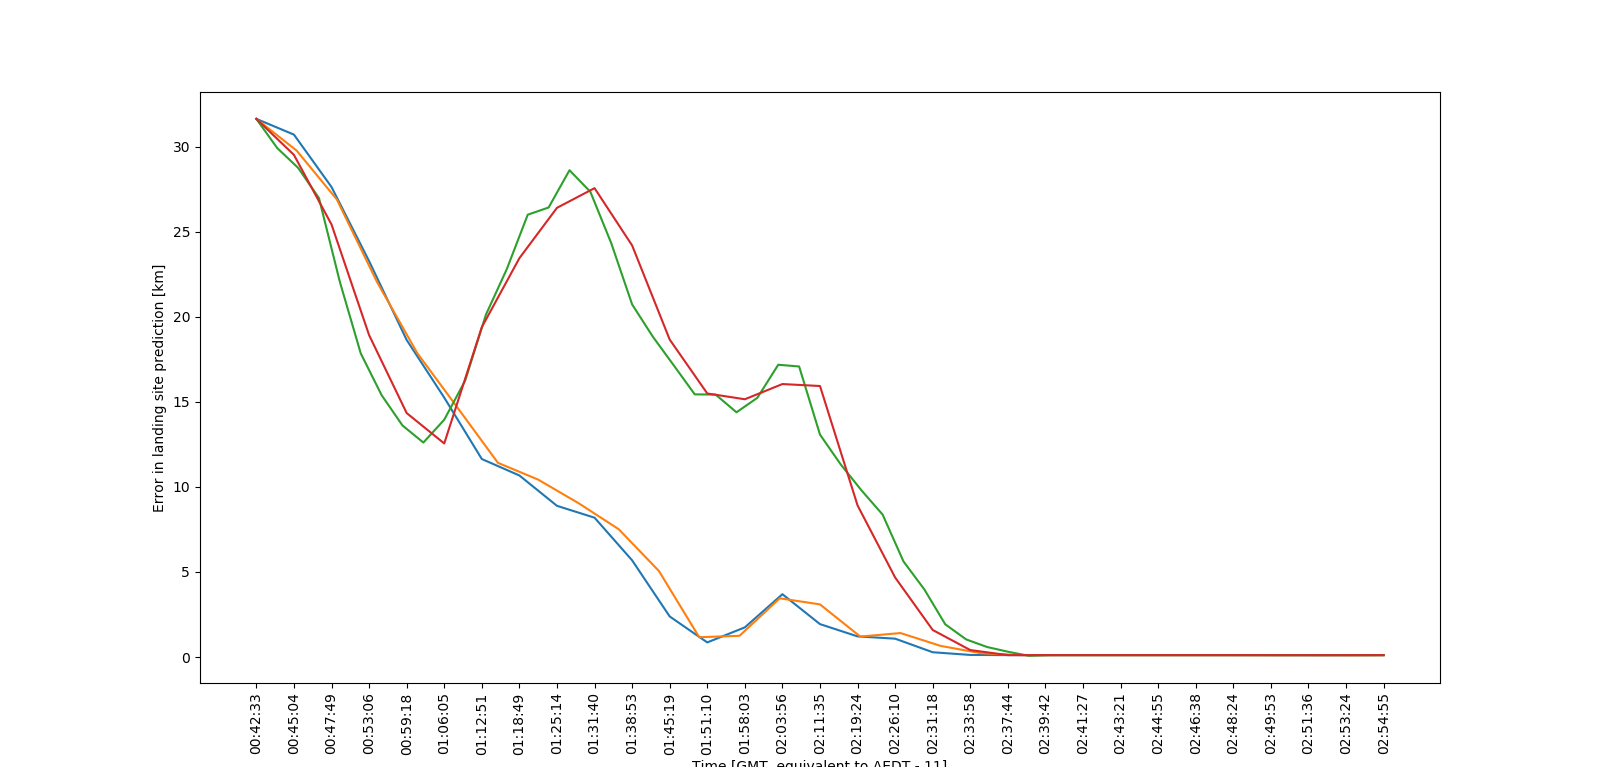
\includegraphics[width=\linewidth]{errors.png}
\end{figure}

As expected,the error at launch is roughly the distance between the launch and landing sites. Given that the program has not yet collected any data about the windbands above it, this makes sense. There is also a larger error around 02:00 - given that this is the period when the balloon is at the peak of its altitude (and thus has the largest number of windbands below it), it makes sense that the uncertainty in the prediction is larger here. \\

There are two major sources of error with using this dataset as a method of testing the prediction algorithm though. The first is that the launch and landing sites of the balloon are already comparatively close together, meaning a prediction algorithm could just return its own latitude and longitude and still be correct to on the order of 30 kilometers. Secondly, due to some issues during the YERRALOON1 launch, very accurate records regarding payload mass, helium mass and balloon mass do not exist. The mass measurements used in this program are derived from the temperature and pressure measurements recorded at the launch site, as well as measuring the size of the balloon on footage from the launch. 

\section{Future Work}

There is much that can still be done to improve the accuracy and usability of the landing site prediction software. As previously discussed, many of the potential issues of the software are obscured by the limitations of the data from the YERRALOON1 flight. Committing to a new HAB launch, or obtaining the telemetry from a prior launch (including vital data such as payload mass and gas mass) is an important next step in testing the accuracy of the prediction software in order to understand when and how it fails. \\

Future iterations of the program might also benefit from having an active connection to a computer on the ground (i.e. the program might be able to make use of data uploaded from the ground computer). For example, this might be useful in cases where the payload is experiencing a large horizontal drift, where angular speed data is less relevant. A more robust program would also be able to handle input data in different formats; this would mean that the prediction system would no longer be reliant on simultaneously running the Ackerman tracker code. Lastly, the program would benefit from the ability to take a more probabilistic approach to the landing prediction algorithm, which would help to quantify the uncertainty in the prediction - for example, the uncertainty in the descent mass of the payload or uncertainty in windspeed might be better modelled using a stochastic rather than deterministic process.

\section{Conclusion}

\newpage

\section{References}

\end{document}